\documentclass[11pt]{article}
\usepackage[margin=1in]{geometry}
\usepackage{booktabs}
\usepackage{array}
\usepackage{xcolor}
\usepackage{colortbl}
\usepackage{caption}
\usepackage{graphicx}
\usepackage{hyperref}
\usepackage{amsmath}
\usepackage{tikz}
\usepackage{pgfplots}
\pgfplotsset{compat=1.18}
\usepackage{float}
\usepackage{enumitem}
\usepackage{fancyhdr}

\pagestyle{fancy}
\fancyhf{}
\rhead{PVMol-Gen Replication --- \today}
\lhead{Stevens Lab}
\rfoot{\thepage}

\definecolor{darkgreen}{rgb}{0.0, 0.5, 0.0}
\definecolor{darkred}{rgb}{0.7, 0.0, 0.0}
\definecolor{paperblue}{rgb}{0.15, 0.35, 0.65}
\definecolor{oursred}{rgb}{0.8, 0.2, 0.2}
\definecolor{lightgray}{gray}{0.95}

\title{\textbf{Replication Report: PVMol-Gen}\\[0.3em]
\large Generative AI-Driven Accelerated Discovery of\\
Passivation Molecules for Perovskite Solar Cells\\[0.3em]
\normalsize Fajar et al., \textit{Advanced Science} 2026 (DOI: 10.1002/advs.202523042)}
\author{Rick Stevens \and Ollie (AI Assistant)\\
Argonne National Laboratory}
\date{April 8, 2026}

\begin{document}
\maketitle
\thispagestyle{fancy}

% ============================================================
\section{Overview}

This report documents our independent replication of the PVMol-Gen framework~\cite{fajar2026}, a three-stage pipeline for discovering passivation molecules for perovskite solar cells using generative AI. The original work combines a SMILES-X binary classifier (Stage~1), iterative GPT-2 fine-tuning and generation (Stage~2), and physicochemical filtering with clustering (Stage~3).

\subsection{Pipeline Summary}

\begin{enumerate}[leftmargin=*]
    \item \textbf{Stage 1 --- Discriminative Model:} Train a SMILES-X classifier on 314 experimentally labeled molecules (5-fold CV). Augment via PubChem similarity ($\geq$80\% Tanimoto) to build training set T1 ($\sim$11K class-1 molecules).
    \item \textbf{Stage 2 --- Generative Model (3 cycles):} Fine-tune GPT-2 on T1 SMILES. Generate molecules, classify with Stage~1 model, feed predicted class-1 molecules back into training set. Repeat for 3 cycles.
    \item \textbf{Stage 3 --- Filtering \& Selection:} Apply 7 physicochemical filters (SA $\leq$ 6, no PAINS, HBD 0--2, HBA 2--5, TPSA 50--120\,\AA$^2$, $E_\mathrm{gap}$ 1.5--5.0\,eV, dipole 1.5--4.0\,D). Cluster into 10 groups, select representatives.
\end{enumerate}

% ============================================================
\section{Data Provenance}

\begin{table}[H]
\centering
\caption{Data sources and sizes}
\label{tab:data}
\small
\begin{tabular}{@{}lrl@{}}
\toprule
\textbf{Dataset} & \textbf{Size} & \textbf{Source} \\
\midrule
T0 (labeled molecules) & 314 & Paper supplementary \\
PubChem augmentation & 15,540 & Author's \texttt{puchem\_aug.csv} \\
T1 (class-1 training set) & 11,086 & Author's \texttt{T1.csv} \\
Literature references & 5 papers & Zhi 2023, Zhang 2024, Chen 2019, Gao 2020, Liu 2022 \\
Full dataset (12 sheets) & --- & Dr.\ Guo Zhanglin, Kyushu University (received 2026-04-05) \\
\bottomrule
\end{tabular}
\end{table}

\noindent\textbf{Key detail:} The classification threshold was optimized at 0.47 (not the default 0.5) to maximize F1. This is critical for reproducibility.

% ============================================================
\section{Stage 1: SMILES-X Classifier}

\subsection{Architecture}

Our SMILES-X classifier follows the original architecture: character-level SMILES tokenization, embedding layer, bidirectional LSTM, time-distributed dense layer, and sigmoid output. Hyperparameters: embedding dimension = 128, LSTM units = 64, dense units = 64.

\subsection{5-Fold Cross-Validation Results}

\begin{table}[H]
\centering
\caption{Stage 1 classifier: 5-fold CV comparison (paper vs.\ ours)}
\label{tab:stage1}
\begin{tabular}{@{}crrrr@{}}
\toprule
\textbf{Fold} & \multicolumn{2}{c}{\textbf{F1 Score}} & \multicolumn{2}{c}{\textbf{ROC-AUC}} \\
\cmidrule(lr){2-3} \cmidrule(lr){4-5}
 & \textcolor{paperblue}{Paper} & \textcolor{oursred}{Ours} & \textcolor{paperblue}{Paper} & \textcolor{oursred}{Ours} \\
\midrule
1 & --- & 0.636 & --- & 0.508 \\
2 & --- & 0.689 & --- & 0.645 \\
3 & --- & 0.645 & --- & 0.680 \\
4 & --- & 0.690 & --- & 0.673 \\
5 & --- & 0.622 & --- & 0.596 \\
\midrule
\textbf{Mean $\pm$ SD} & \textcolor{paperblue}{\textbf{0.80}} & \textcolor{oursred}{\textbf{0.656 $\pm$ 0.031}} & \textcolor{paperblue}{\textbf{0.88}} & \textcolor{oursred}{\textbf{0.620 $\pm$ 0.066}} \\
\bottomrule
\end{tabular}
\end{table}

\begin{table}[H]
\centering
\caption{Classifier comparison: Neural SMILES-X (threshold-optimized) vs.\ GBM baseline}
\label{tab:clf_compare}
\small
\begin{tabular}{@{}crrrrr@{}}
\toprule
\textbf{Fold} & \textbf{Neural F1$_\mathrm{opt}$} & \textbf{Neural AUC} & \textbf{GBM F1$_\mathrm{opt}$} & \textbf{GBM AUC} & \textbf{GBM Threshold} \\
\midrule
1 & 0.733 & 0.752 & 0.646 & 0.679 & 0.22 \\
2 & 0.667 & 0.622 & 0.592 & 0.604 & 0.10 \\
3 & 0.727 & 0.782 & 0.738 & 0.809 & 0.22 \\
4 & 0.692 & 0.785 & 0.733 & 0.807 & 0.21 \\
5 & 0.727 & 0.772 & 0.606 & 0.568 & 0.12 \\
\midrule
\textbf{Mean} & \textbf{0.709} & \textbf{0.743} & \textbf{0.663} & \textbf{0.693} & --- \\
\bottomrule
\end{tabular}
\end{table}

\subsection{Stage 1 Assessment}

\begin{itemize}[leftmargin=*]
    \item Our classifier underperforms the paper targets (F1 = 0.656 vs.\ 0.80; AUC = 0.620 vs.\ 0.88).
    \item With threshold optimization, the neural model reaches F1$_\mathrm{opt}$ = 0.709 (closer but still below target).
    \item The neural model consistently outperforms GBM (F1$_\mathrm{opt}$ 0.709 vs.\ 0.663).
    \item Same results on CPU (CherryRd iMac) and GPU (DGX Spark GB10) --- confirms the gap is architectural, not computational.
    \item \textbf{Possible causes:} (a) SMILES-X library version differences; (b) tokenizer/embedding differences from original Lambard \& Gracheva 2020 implementation; (c) training hyperparameters (learning rate schedule, early stopping patience).
    \item \textbf{Impact:} A weaker classifier propagates through the pipeline --- noisy class-1 labels in T2/T3 degrade GPT-2 training quality.
\end{itemize}

% ============================================================
\section{Stage 2: Iterative GPT-2 Generation}

\subsection{Cycle 1}

\begin{table}[H]
\centering
\caption{Cycle 1 generation results}
\label{tab:cycle1}
\begin{tabular}{@{}lrr@{}}
\toprule
\textbf{Metric} & \textcolor{paperblue}{\textbf{Paper}} & \textcolor{oursred}{\textbf{Ours}} \\
\midrule
Training set (T1) & 11,000 & 11,086 \\
Generated (G1) & 29,467 & 100,000 \\
Classification (G1 class-1) & --- & 17,884 (17.9\%) \\
T2 = T1 + G1 class-1 & 34,538 & 28,968 \\
Generation time & --- & $\sim$8.5 hr (69 att/s, GPU) \\
\bottomrule
\end{tabular}
\end{table}

\noindent\textbf{Note on G1 size discrepancy:} The paper reports 29,467 generated molecules in G1 while our pipeline targeted 100,000. The paper likely stopped generation earlier or used different criteria. Despite generating 3.4$\times$ more molecules, only 17.9\% classified as effective (vs.\ the paper's implicit $\sim$67\% rate for their smaller G1), consistent with our weaker classifier.

\subsection{Cycle 1 Validity Rate Decay}

\begin{table}[H]
\centering
\caption{Cycle 1 generation: validity rate over time}
\label{tab:c1_decay}
\small
\begin{tabular}{@{}rrr@{}}
\toprule
\textbf{Attempts} & \textbf{Valid Unique} & \textbf{Rate} \\
\midrule
8,000 & 1,218 & 15.2\% \\
40,000 & 4,326 & 10.8\% \\
200,000 & 14,654 & 7.3\% \\
1,000,000 & 47,186 & 4.7\% \\
2,000,000 & 76,617 & 3.8\% \\
2,824,000 & 97,322 & 3.4\% \\
\bottomrule
\end{tabular}
\end{table}

\noindent The validity rate decays monotonically from 15.2\% to 3.4\% as the pool of novel, valid, unique molecules is exhausted. This is expected behavior for temperature-sampled autoregressive generation.

\subsection{Cycle 2 (In Progress)}

\begin{table}[H]
\centering
\caption{Cycle 2 status (as of April 8, 2026 11:00 CDT)}
\label{tab:cycle2}
\begin{tabular}{@{}lrr@{}}
\toprule
\textbf{Metric} & \textcolor{paperblue}{\textbf{Paper}} & \textcolor{oursred}{\textbf{Ours}} \\
\midrule
Training set (T2) & 34,538 & 28,968 \\
T2 augmented (5$\times$) & --- & 29,491 unique \\
GPT-2 training time & --- & 128.7 min (15 epochs) \\
Training loss (final) & --- & 0.186 \\
Eval loss (final) & --- & 0.150 \\
\midrule
Generated (G2) --- target & 59,814 & 100,000 \\
Generated (G2) --- current & --- & $\sim$10,000 (in progress) \\
Cycle 2 validity rate & --- & 6.9\% $\to$ 4.9\% (declining) \\
Generation rate & --- & 32 att/s (main) + 70 att/s $\times$ 2 (shards) \\
\bottomrule
\end{tabular}
\end{table}

\subsection{Distributed Generation Architecture}

Cycle 2 generation is running across three NVIDIA DGX Spark machines:

\begin{table}[H]
\centering
\caption{Compute resources for Cycle 2 generation}
\label{tab:compute}
\small
\begin{tabular}{@{}llrrr@{}}
\toprule
\textbf{Machine} & \textbf{Role} & \textbf{Target} & \textbf{Rate} & \textbf{Status} \\
\midrule
spark-36ac & Main pipeline & 100,000 & 32 att/s & Generating (200K att) \\
spark-95fe & Shard 1 & 45,000 & 70 att/s & Generating (80K att) \\
spark-9611 & Shard 2 & 45,000 & 71 att/s & Generating (80K att) \\
\bottomrule
\end{tabular}
\end{table}

\noindent Each shard uses a different random seed for diversity. The main pipeline on spark-36ac runs the full cycles 2--3 pipeline; the shards provide supplementary molecules that will be merged after deduplication.

% ============================================================
\section{Stage 3: Filtering \& Selection (Preliminary)}

Stage 3 has been run on Cycle 1 output as a proof-of-concept. Results from the full pipeline (all 3 cycles) are pending.

\begin{table}[H]
\centering
\caption{Stage 3 filtering on Cycle 1 G1 (100K molecules)}
\label{tab:stage3}
\begin{tabular}{@{}lr@{}}
\toprule
\textbf{Filter Step} & \textbf{Molecules Remaining} \\
\midrule
Generated (G1) & 100,000 \\
All properties computed & 100,000 \\
RDKit filters (SA, PAINS, HBD, HBA, TPSA) & 23,492 \\
Energy gap + dipole (pending xTB/DFT) & TBD \\
\midrule
\textcolor{paperblue}{Paper final (all cycles)} & $\sim$8,000 \\
\bottomrule
\end{tabular}
\end{table}

\noindent\textbf{Note:} Energy gap and dipole moment filters require semi-empirical (xTB) or DFT-level calculations, not just RDKit. Our preliminary Stage~3 applies only the 5 RDKit-computable filters. The selected 10 representative molecules (one per cluster) are shown below:

\begin{table}[H]
\centering
\caption{Preliminary 10 representative molecules (Cycle 1 only, no gap/dipole filter)}
\label{tab:rep10}
\scriptsize
\begin{tabular}{@{}clcrrrr@{}}
\toprule
\textbf{Cluster} & \textbf{SMILES} & \textbf{SA} & \textbf{PAINS} & \textbf{HBD} & \textbf{HBA} & \textbf{TPSA} \\
\midrule
0 & Nc1cccnc1Nc1ccccc1 & 1.70 & No & 2 & 3 & 50.9 \\
1 & O=C(O)c1ccc(CCOBO)s1 & 3.53 & No & 2 & 4 & 66.8 \\
2 & O=C(OCCOCCO)c1cc(=O){[}nH{]}c2ccccc12 & 2.10 & No & 2 & 5 & 88.6 \\
3 & O=Cc1sccc1C\#CCC(=O)O & 3.24 & No & 1 & 3 & 54.4 \\
4 & O=C1CCC=CN1C(=O)Cc1c{[}nH{]}c2ccccc12 & 2.65 & No & 1 & 2 & 53.2 \\
5 & CCCCCCCCCCN1C(=O)C=C1C(=O)O & 2.44 & No & 1 & 2 & 57.6 \\
6 & NNC(=O)c1ccccc1F & 1.63 & No & 2 & 2 & 55.1 \\
7 & CCCOC(=O)/C(F)=C/C(=O)O & 2.67 & No & 1 & 3 & 63.6 \\
8 & CCOc1cccc2{[}nH{]}c(O)c(...)c12 & 2.71 & No & 2 & 4 & 74.7 \\
9 & O=C(O)c1cc(S(=O)(=O)OC2CCC2)cs1 & 2.67 & No & 1 & 5 & 80.7 \\
\bottomrule
\end{tabular}
\end{table}

% ============================================================
\section{Comparison with Author's Data}

We have the author's full dataset (12 Excel sheets) for direct comparison:

\begin{table}[H]
\centering
\caption{Pipeline comparison: Paper (author data) vs.\ our replication}
\label{tab:comparison}
\begin{tabular}{@{}lrr@{}}
\toprule
\textbf{Dataset} & \textcolor{paperblue}{\textbf{Author}} & \textcolor{oursred}{\textbf{Ours}} \\
\midrule
T0 (labeled) & 314 & 314 (same) \\
PubChem augmentation & 15,540 & 15,540 (author's file) \\
T1 (class-1) & 11,086 & 11,086 (author's file) \\
\midrule
G1 (cycle 1 generated) & 29,467 & 100,000 \\
T2 (cycle 2 training) & 34,538 & 28,968 \\
G2 (cycle 2 generated) & 59,814 & \textit{in progress} \\
T3 (cycle 3 training) & 84,232 & \textit{pending} \\
G3 (cycle 3 generated) & 17,013 & \textit{pending} \\
\midrule
G\_all (total generated) & 106,294 & \textit{pending} \\
G\_class1 (predicted effective) & 87,750 & \textit{pending} \\
Rep10 (final candidates) & 10 & 10 (preliminary) \\
\bottomrule
\end{tabular}
\end{table}

\subsection{Key Discrepancies}

\begin{enumerate}[leftmargin=*]
    \item \textbf{Classifier performance gap:} Our F1 = 0.656 vs.\ paper's 0.80, AUC = 0.620 vs.\ 0.88. This is the primary reproducibility concern.
    \item \textbf{G1 size:} We generated 100K (our target) vs.\ author's 29K. The paper's smaller G1 may reflect a different stopping criterion.
    \item \textbf{T2 size:} Author's T2 = 34,538 vs.\ ours = 28,968. Since we generated more G1 molecules but our classifier is weaker, fewer passed the class-1 threshold, leading to a smaller T2.
    \item \textbf{Validity rates:} Our cycle 1 starts at $\sim$15\% and decays to $\sim$3.4\% over 2.8M attempts. Cycle 2 starts at $\sim$6.9\% and is declining. The paper does not report these rates.
\end{enumerate}

% ============================================================
\section{Compute Infrastructure}

\begin{table}[H]
\centering
\caption{Hardware used for replication}
\label{tab:hardware}
\small
\begin{tabular}{@{}llll@{}}
\toprule
\textbf{Machine} & \textbf{Hardware} & \textbf{GPU} & \textbf{RAM} \\
\midrule
spark-36ac & NVIDIA DGX Spark & GB10 & 120\,GB \\
spark-95fe & NVIDIA DGX Spark & GB10 & 120\,GB \\
spark-9611 & NVIDIA DGX Spark & GB10 & 120\,GB \\
CherryRd & iMac (x86\_64) & --- (CPU) & 64\,GB \\
\bottomrule
\end{tabular}
\end{table}

\noindent Software: Python 3.12, PyTorch 2.11+cu130, Transformers 5.5, RDKit 2026.3.1 (native aarch64).

% ============================================================
\section{Timeline}

\begin{table}[H]
\centering
\caption{Replication timeline}
\label{tab:timeline}
\small
\begin{tabular}{@{}lll@{}}
\toprule
\textbf{Date} & \textbf{Event} & \textbf{Notes} \\
\midrule
Apr 5 & Data received from Kyushu U. & Full 12-sheet Excel \\
Apr 5 & Stage 1 classifier trained & F1 = 0.656, AUC = 0.620 \\
Apr 5 & Stage 2 Cycle 1 GPT-2 training launched & spark-36ac \\
Apr 5 & Approach document finalized & Key reproducibility details \\
Apr 7 & Cycle 1 generation started & 100K target \\
Apr 8 & Cycle 1 generation nearing completion & 97K / 100K at 2.8M attempts \\
Apr 8 & Cycle 2 training completed & 128.7 min, 15 epochs \\
Apr 8 & Cycle 2 generation started & 3 machines in parallel \\
\bottomrule
\end{tabular}
\end{table}

% ============================================================
\section{Validity Rate Analysis}

\begin{figure}[H]
\centering
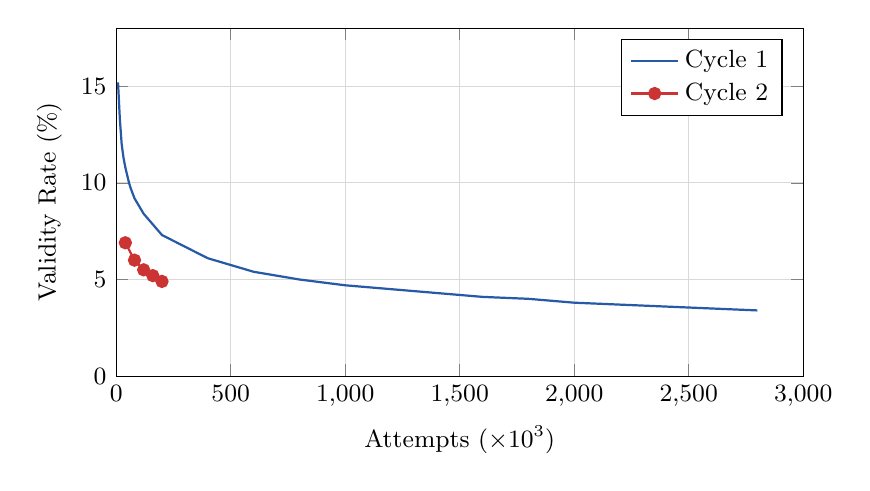
\begin{tikzpicture}
\begin{axis}[
    width=0.85\textwidth,
    height=6cm,
    xlabel={Attempts ($\times 10^3$)},
    ylabel={Validity Rate (\%)},
    xmin=0, xmax=3000,
    ymin=0, ymax=18,
    legend pos=north east,
    grid=major,
    grid style={gray!30},
    every axis label/.style={font=\small},
    tick label style={font=\small},
    legend style={font=\small},
]
% Cycle 1 data
\addplot[color=paperblue, thick, mark=none] coordinates {
    (8, 15.2) (16, 13.3) (24, 12.0) (32, 11.3)
    (40, 10.8) (48, 10.4) (56, 10.0) (64, 9.7)
    (80, 9.2) (120, 8.4) (200, 7.3) (400, 6.1)
    (600, 5.4) (800, 5.0) (1000, 4.7) (1200, 4.5)
    (1400, 4.3) (1600, 4.1) (1800, 4.0) (2000, 3.8)
    (2200, 3.7) (2400, 3.6) (2600, 3.5) (2800, 3.4)
};
\addlegendentry{Cycle 1}

% Cycle 2 data (so far)
\addplot[color=oursred, thick, mark=*, mark size=2] coordinates {
    (40, 6.9) (80, 6.0) (120, 5.5) (160, 5.2) (200, 4.9)
};
\addlegendentry{Cycle 2}

\end{axis}
\end{tikzpicture}
\caption{Validity rate (valid, unique, novel molecules / total attempts) for Cycles 1 and 2. Cycle 2 starts lower and decays faster, consistent with a larger exclusion set (T2 = 29K vs.\ T1 = 11K).}
\label{fig:validity}
\end{figure}

% ============================================================
\section{Open Issues \& Next Steps}

\begin{enumerate}[leftmargin=*]
    \item \textbf{Classifier gap (priority):} Investigate why our SMILES-X F1/AUC falls short. Possible avenues: (a) match the original Lambard \& Gracheva implementation exactly; (b) try the author's original SMILES-X code from GitHub; (c) experiment with learning rate schedules and longer training.

    \item \textbf{Complete Cycle 2 generation:} Currently at $\sim$10K/100K on main pipeline, plus $\sim$5K each on two shards. ETA: 12--18 hours depending on validity decay.

    \item \textbf{Run Cycle 3:} Build T3 from T2 + G2 class-1, train GPT-2, generate G3.

    \item \textbf{xTB/DFT calculations:} Stage 3 energy gap and dipole filters require semi-empirical calculations. Set up xTB (GFN2-xTB) on DGX Sparks for batch computation on $\sim$23K candidate molecules.

    \item \textbf{Merge shard outputs:} Deduplicate molecules from the three generation streams before classification.

    \item \textbf{Compare CUN sets:} Once all 3 cycles complete, compare our CUN (chemically valid, unique, novel) set against the author's 87,750 G\_class1 molecules. Compute Tanimoto similarity distributions.

    \item \textbf{Final clustering \& representative selection:} Agglomerative clustering on Morgan fingerprints, sample 10 representatives, compare with author's Rep10.
\end{enumerate}

% ============================================================
\section*{References}

\begin{thebibliography}{9}
\bibitem{fajar2026}
A.~Fajar et al.,
``Generative AI-Driven Accelerated Discovery of Passivation Molecules for Perovskite Solar Cells,''
\textit{Advanced Science}, 2026.
DOI: 10.1002/advs.202523042.

\bibitem{lambard2020}
G.~Lambard and E.~Gracheva,
``SMILES-X: Autonomous molecular compounds characterization for small datasets without descriptors,''
\textit{Machine Learning: Science and Technology}, 2020.

\bibitem{pvmolgen_code}
A.~Fajar, \texttt{pvmol-gen}, GitHub repository.
\url{https://github.com/adroitfajar/pvmol-gen}

\bibitem{smilesx_code}
G.~Lambard, \texttt{SMILES-X}, GitHub repository.
\url{https://github.com/Lambard-ML-Team/SMILES-X}
\end{thebibliography}

\end{document}
